\section{Beispiel 3: Charge Balancer}

Die gegebene Schaltung wurde durch folgende Elemente erweitert:

\begin{itemize}
 \item ein 4-bit Synchronz"ahler U2 (74293), der den Takt des D-Flipflops verwendet und durchgehend von 0 bis 15 z"ahlt (der Z"ahler l"auft dann "uber und beginnt wieder bei 0)
 \item ein 4-bit Synchronz"ahler U3 (74293), der den Ausgang des NAND-Gatters als Takt verwendet und so die Impulse der Schaltung z"ahlt
 \item ein 4-bit Latch U4 (74176), das jedes Mal beim Erreichen des letzten Taktes von U2 (Z"ahlerstand 15) den aktuellen Z"ahlerstand von U3 speichert
 \item Logik, die beim Erreichen des letzten Taktschritts in der positiven H"alfte des Takts das Latch U4 l"adt
 \item Logik, die beim Erreichen des letzten Taktschritts in der negativen H"alfte des Takts den Z"ahler U3 zur"ucksetzt
\end{itemize}

\begin{figure}[ht]
 \centering
 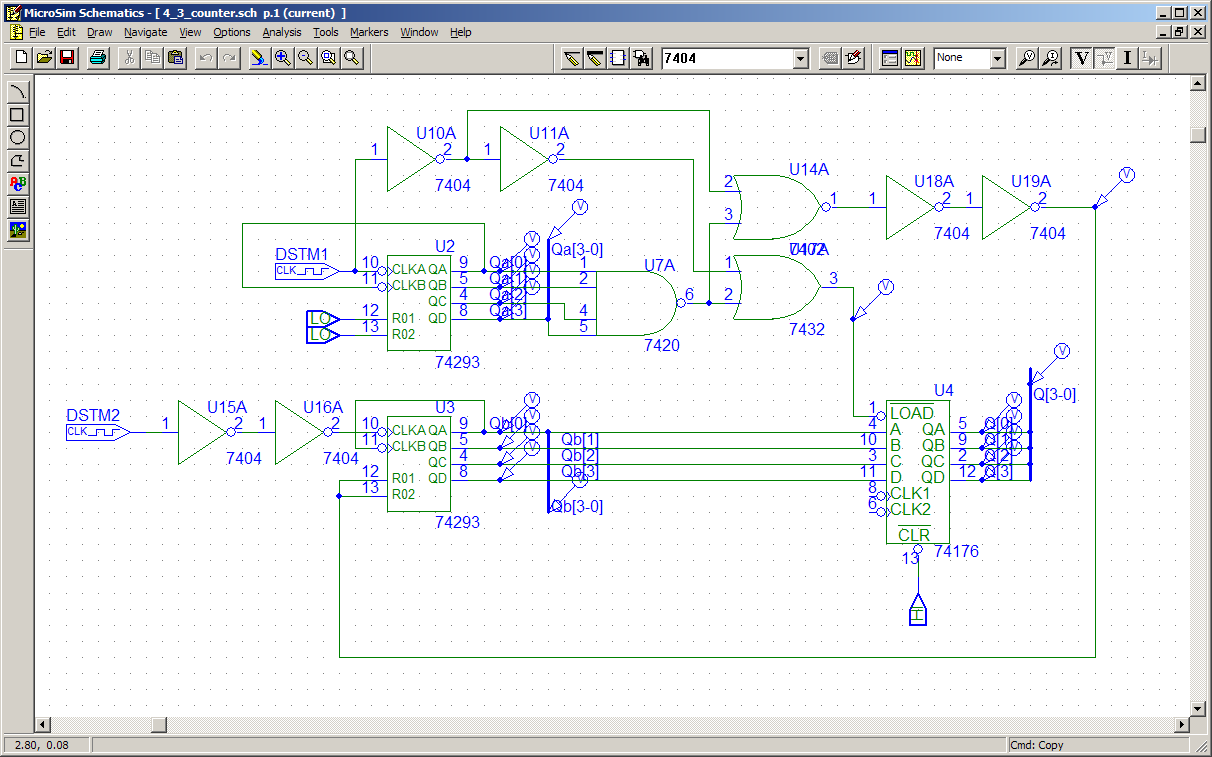
\includegraphics[width=\textwidth]{./img/4_3_counter_schem.PNG}
 \caption{Z"ahler f"ur Beispiel 3}
 \label{fig:4_3_counter_schem}
\end{figure}


Diese Erweiterungen wurden zuerst seperat simuliert (siehe Abbildung~\ref{fig:4_3_counter_schem}). Dabei muss besonders darauf geachtet werden, dass sich durch die Propagation Delays die Signale nicht so verschieben, dass es zu undefinierten Zust"anden kommt. Erreicht wurde das durch eine zus"atzliche Verz"ogerung durch 2 hintereinandergeschaltene Inverter.

Abbildung~\ref{fig:4_3_counter} stellt die Funtionsweise der Schaltung dar. U2 z"ahlt immer von 0 bis 15, U3 z"ahlt mit einem anderen Takt hoch. Erreicht U2 den Wert 15, wird der Wert von U3 im Latch U4 gespeichert und U3 zur"uckgesetzt.

\begin{figure}[ht]
 \centering
 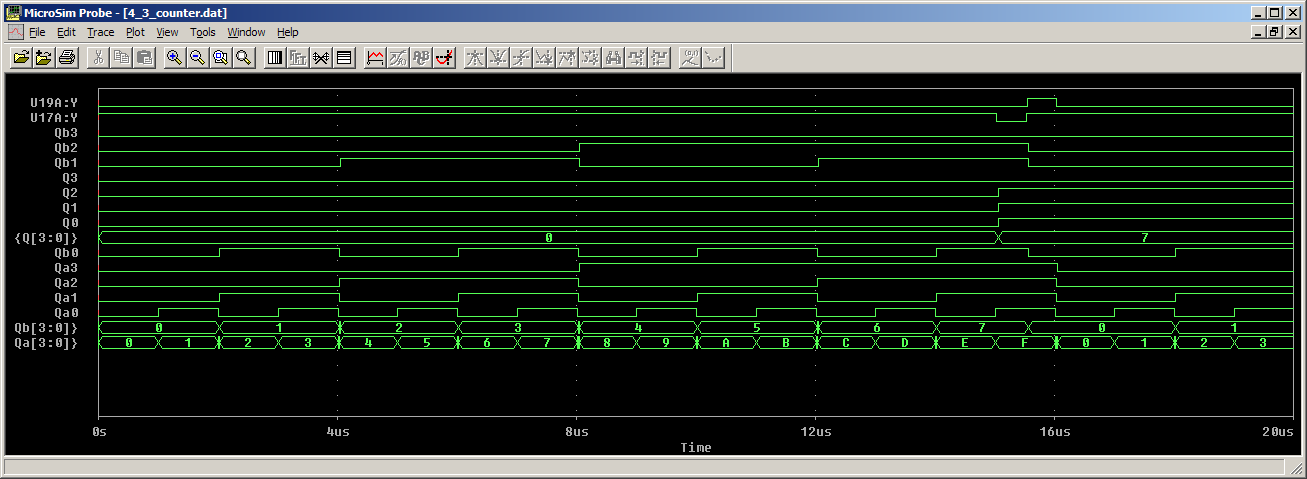
\includegraphics[width=\textwidth]{./img/4_3_counter.PNG}
 \caption{Simulation des Z"ahlers f"ur Beispiel 3}
 \label{fig:4_3_counter}
\end{figure}

Die Schaltung wurde dem gegebenen Charge Balancer hinzugef"ugt und wiederum getestet (siehe Abbildung~\ref{fig:4_3_schem}). Wegen leicht verschobenen Takt- und Signalflanken mussten wieder 2 Inverter hinzugef"ugt werden. Die Simulation mit typischen Timings funktionierte (siehe Abbildung~\ref{fig:4_3}), das Springen des Ausgangswerts ist darauf zur"uckzuf"uhren, dass die Impulse nicht genau zu jedem 16. Takt auftreten, und deswegen pro Periode von 16 Takten ein Takt mehr oder weniger aufgenommen werden kann (dieser Fall tritt jedoch nur selten und nur eine Periode lang auf). Au\ss{}erdem erkennt man die Einschwingphase der Schaltung.

\begin{figure}[ht]
 \centering
 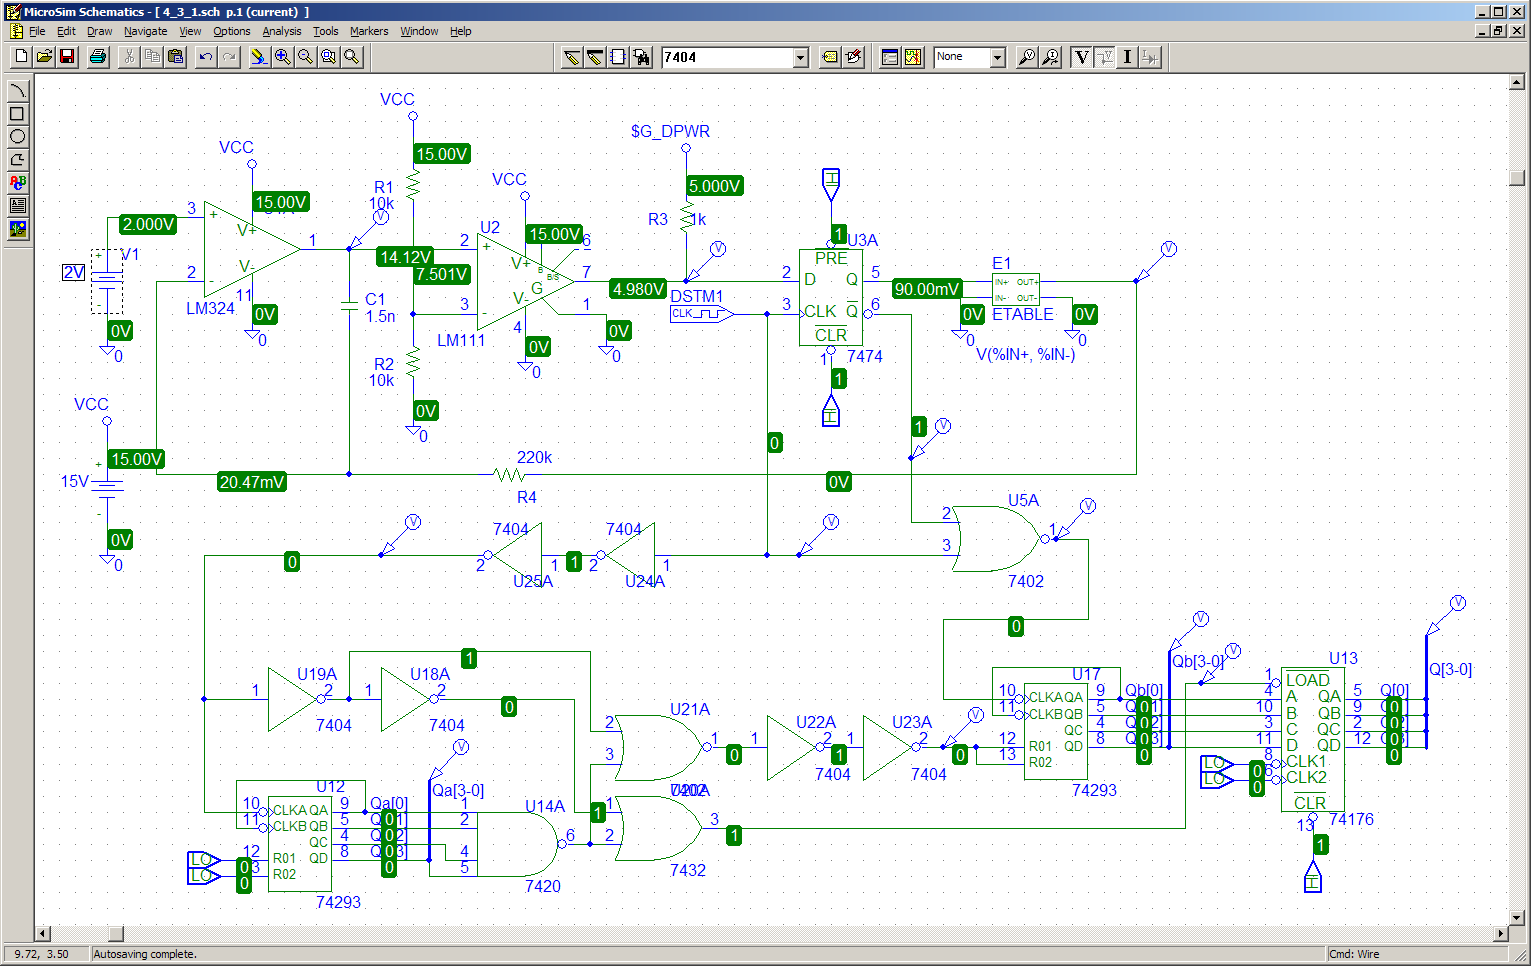
\includegraphics[width=\textwidth]{./img/4_3_schem.PNG}
 \caption{Vollst"andige Schaltung f"ur Beispiel 3}
 \label{fig:4_3_schem}
\end{figure}

\begin{figure}[ht]
 \centering
 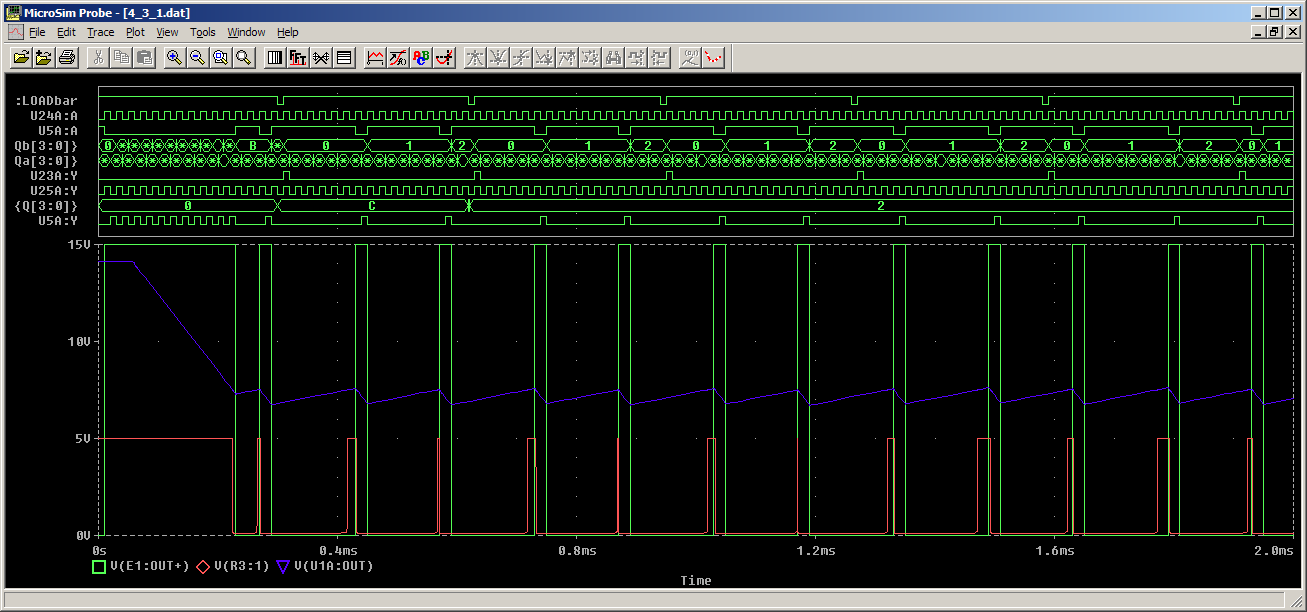
\includegraphics[width=\textwidth]{./img/4_3.PNG}
 \caption{Simulation der vollst"andigen Schaltung f"ur Beispiel 3}
 \label{fig:4_3}
\end{figure}

Bei der Worst-Case-Simulation funktionierte die Schaltung "uberhaupt nicht mehr, da die Takt- und Signalimpulse oft so stark versetzt waren, dass es zu undefinierten Zust"anden kam. Auch durch l"angeres Herumprobieren und Umbauen der Schaltung verbesserte sich die Situation nicht.


\clearpage
\section{Beispiel 4: Temperaturabh"angige L"uftersteuerung}

Passend zu den hohen Temperaturen wurde als letztes Beispiel eine L"uftersteuerung entworfen und simuliert, die aus der aktuellen Temperatur, gemessen mit einer Diode, ein PWM-Signal erzeugt, mit dem "uber einen MOSFET ein L"ufter angesteuert werden kann.

\begin{figure}[ht]
 \centering
 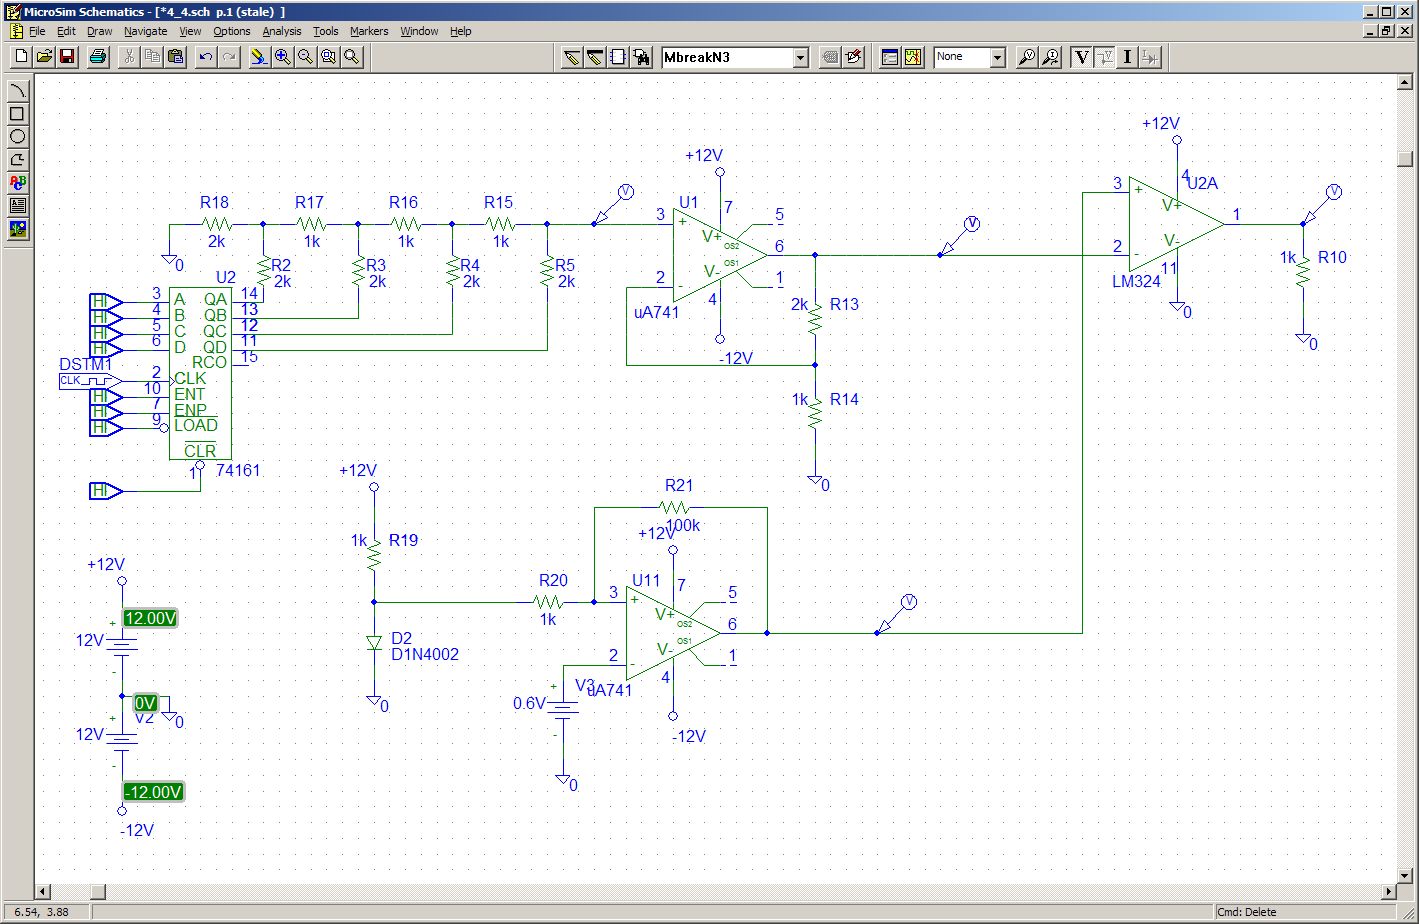
\includegraphics[width=\textwidth]{./img/4_4_schem.PNG}
 \caption{Schaltung der L"uftersteuerung}
 \label{fig:4_4_schem}
\end{figure}

Zu erst muss aus der Ausgangsspannung der Diode eine absolute Temperatur errechnet werden. Ausgenutzt wurde die "Anderung der Diodenflussspannung von $-1.7\frac{mV}{K}$. Mit einem invertierenden Verst"arker wurde die Flussspannung der Diode (durch Simulation ermittelt, ca. 0.6V) subtrahiert und die "Anderung der Flussspannung auf brauchbare Werte verst"arkt (siehe Abbildung~\ref{fig:4_4_schem}). Der Offset und die Verst"arkung k"onnen so berechnet werden, dass sich im Temperaturbereich von 20 bis 40 Grad Celsius eine Spannung von 0V bis 10V ergibt.

F"ur die Erzeugung der PWM wurde mit Hilfe eines Z"ahlers ein Rampensignal erzeugt. Ein 4-bit Synchronz"ahler (74293) z"ahlt immer wieder von 0 bis 15 und l"auft dann wieder "uber. Am Ausgang des Z"ahlers befindet sich eine Widerstandsleiter, durch die eine analoge Spannung zwischen 0 und 5V erzeugt wird. Diese Spannung ist s"agezahnf"ormig. Mit einem nichtinvertierenden Verst"arker wird diese Spannung dann an den gew"unschten Bereich angepasst.

Ein Komparator vergleicht die S"agezahnspannung und die Temperaturspannung. Je nach H"ohe der Temperaturspannung schaltet der Komparator um, sobald die Rampe die Temperaturspannung "uberschreitet. Dadurch ist die high-Dauer des Komparatorausgangs je l"anger, umso h"oher die Temperaturspannung ist. Abbildung~\ref{fig:4_4_2V} zeigt das Verhalten der Schaltung bei einer niedrigen Temperatur, Abbildung~\ref{fig:4_4_7V} zeigt das Verhalten bei einer h"oheren Temperatur. Am Ausgang k"onnte sich ein n-Kanal MOSFET befinden, der in dieser Zeit einen L"ufter einschaltet. Dadurch ergibt sich eine einfache Temperatursteuerung, die die L"ufterdrehzahl an die Temperatur anpasst.

\begin{figure}[ht]
 \centering
 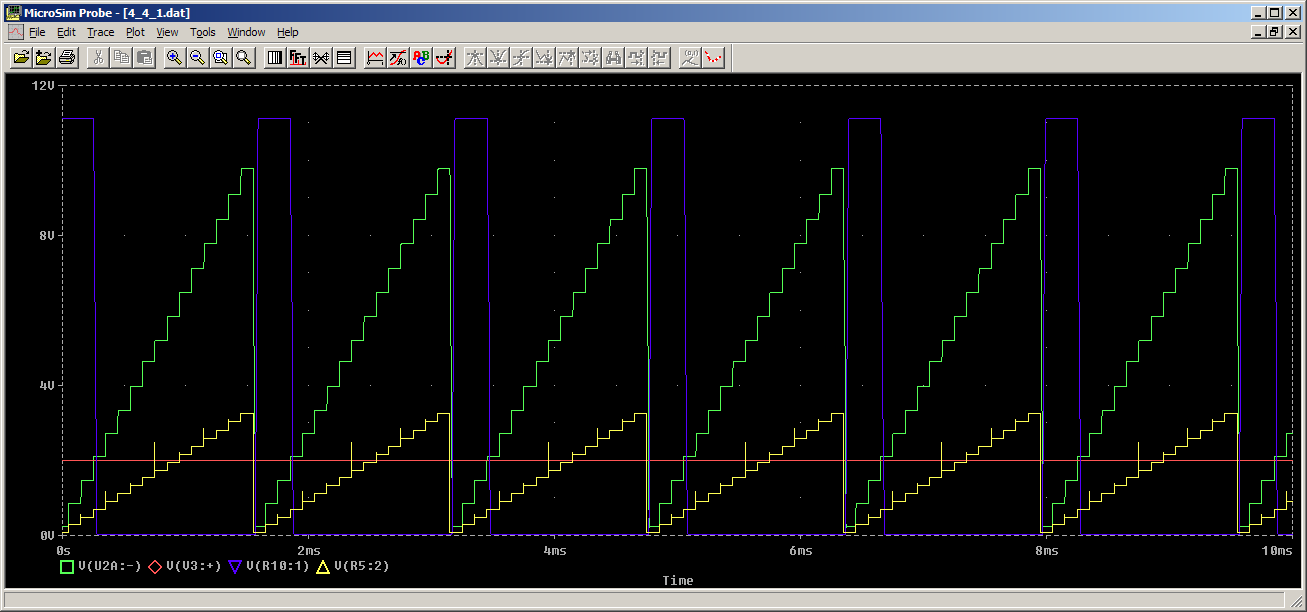
\includegraphics[width=\textwidth]{./img/4_4_2V.PNG}
 \caption{Verhalten der L"uftersteuerung f"ur eine Temperaturspannung von 2V}
 \label{fig:4_4_2V}
\end{figure}

\begin{figure}[ht]
 \centering
 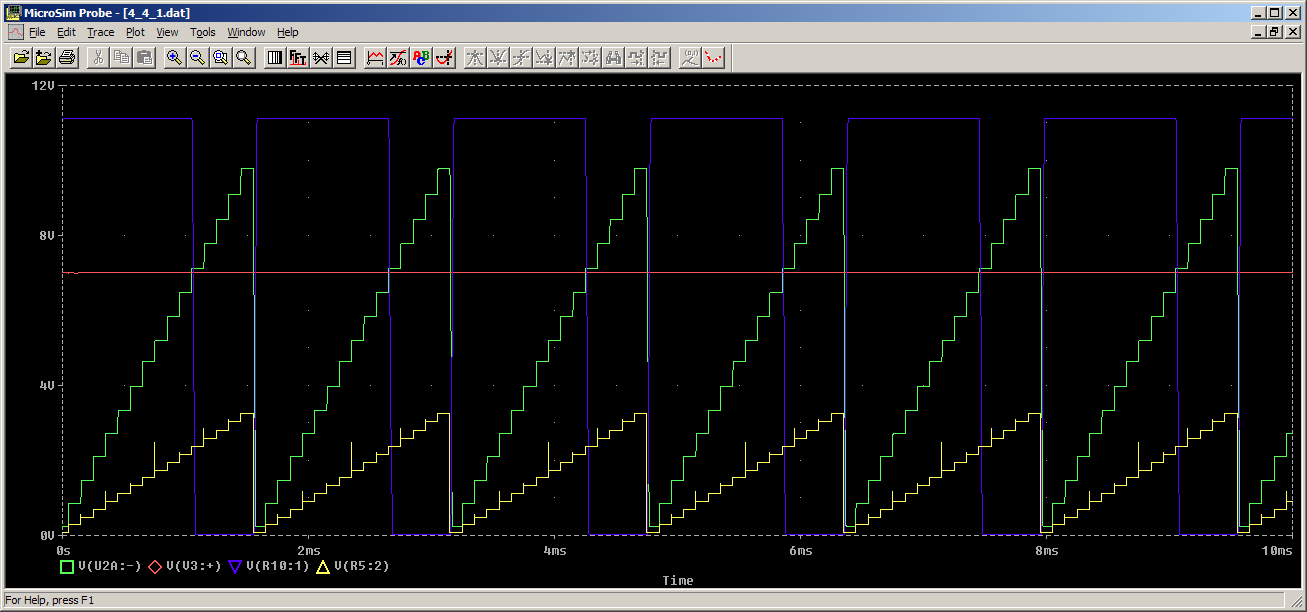
\includegraphics[width=\textwidth]{./img/4_4_7V.PNG}
 \caption{Verhalten der L"uftersteuerung f"ur eine Temperaturspannung von 7V}
 \label{fig:4_4_7V}
\end{figure}

Leider konnten wir die gesamte Schaltung nicht mit der verwendeten Version von PSpice simulieren, da die Anzahl der Nodes zu hoch f"ur die Studentenversion war. Deswegen wurde nur eine vereinfachte Version simuliert, bei der die Erzeugung einer Temperaturspannung durch eine Spannungsquelle ersetzt wurde (siehe Abbildung~\ref{fig:4_4_1_schem}).

\begin{figure}[ht]
 \centering
 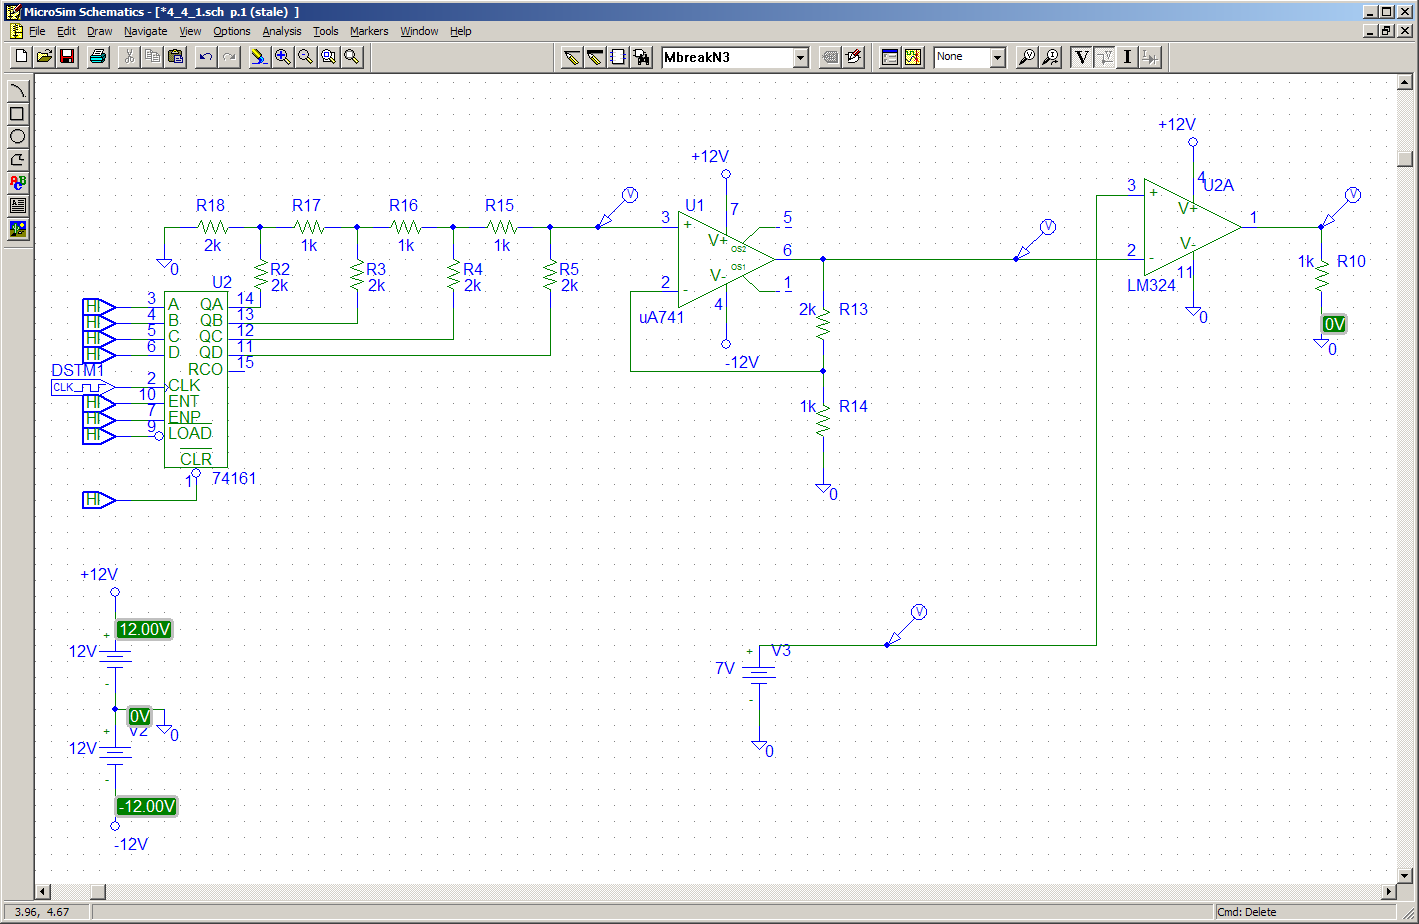
\includegraphics[width=\textwidth]{./img/4_4_1_schem.PNG}
 \caption{Vereinfachte Schaltung zur Simulation mit PSpice}
 \label{fig:4_4_1_schem}
\end{figure}
